\chapter{Questo è un capitolo}

\lipsum[1]

\section{Questa è una sezione}

\lipsum[2]

\subsection{Questa è una sottosezione}

\lipsum[3]

\subsubsection{Questa è una sotto-sottosezione}

\lipsum[4]

É possibile riferire l'immagine, una volta assegnatagli una label, tramite il comando \texttt{\textbackslash autoref\{fig:immagine\}}, ottenendo il seguente risultato: \autoref{fig:immagine}.

\begin{figure}
    \centering
    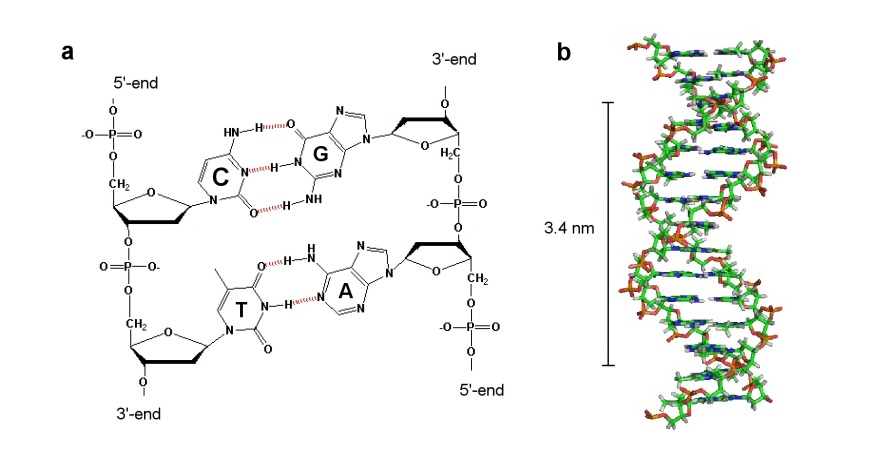
\includegraphics[width=0.8\textwidth]{images/Chapter1/immagine.jpg} % width= 0.8\textwidth
    \caption{Questa è un'immagine} 
    \label{fig:immagine} % this internally labels the figure for future referencing.
\end{figure}

Questa è una citazione \cite{warstadt2020blimp}.
Questa è una citazione "regular in text citation" \citet{warstadt2020blimp}.  % or \cite{<key>}
Questa è una citazione tra parentesi \citep{warstadt2020blimp}
Questa è un'altra citazione \citep{wei2021frequency}
Listing bibliography entries \citep{hu2020systematic, lau2020furiously,  sprouse2016experimental}

\subsubsection{Questa è un'altra sottosezionelipsum}

Quello che segue è un esempio di codice. E' possibile modificare il linguaggio per il synyax highlight, aggiungere parole chiave... E' tutto disponibile nella guida del pacchetto \texttt{listings}.

\lstinputlisting[language=C++]{listings/Capitolo1/code1.cpp} 

\section{Misc notes with refs}

“NATURAL LANGUAGE DOES NOT MAXIMIZE PROBABILITY” 
“Why is human-written text not the most probable text? We conjecture that this is an intrinsic property of human language. Language models that assign probabilities one word at a time without a global model of the text will have trouble capturing this effect. Grice’s Maxims of Communication (Grice, 1975) show that people optimize against stating the obvious. Thus, making every word as predictable as possible will be disfavored. This makes solving the problem simply by training larger models or improving neural architectures using standard per-word learning objectives unlikely: such models are forced to favor the lowest common denominator, rather than informative language.” 
\citep{holtzman2019curious}

Repeated exposure to a type of island construct will increase its perceived acceptability 
\citep{chaves2014subject}

Targed ..syntactic tests on modern language models seem to have started with \citet{linzen2016assessing}, while the use of psycholinguistic tests for this seem to have started with \citet{futrell2018rnns}.

\subsection{Sottosezione con una tabella}

La tabella si indirizza sempre con l'uso di una label, ottenendo il risultato \autoref{tab:labelTabella}.

\begin{table}
    \caption{Una simpatica tabella!}\label{tab:labelTabella}
    \begin{center}
    \begin{tabular}{c|c|c|c}
        \textbf{Colonna 1} & \textbf{Colonna 2} & \textbf{Colonna 3} & \textbf{Colonna 4} \\
        \hline
            $3$      & $24$     & $24$    & $29$ \\ 
            $36$     & $31$     & $49$    & $39$ \\ 
            $32$     & $41$     & $59$    & $57$ \\ 
            $34$     & $60$     & $79$    & $74$ \\ 
            $328$    & $96$     & $194$   & $99$ \\ 
            $356$    & $117$    & $297$   & $149$ \\ 
            $312$    & $315$    & $293$   & $242$ \\ 
            $3024$   & $184$    & $253$   & $019$ \\ 
            $3048$   & $7795$   & $253$   & $077$ \\ 
            $3096$   & $7767$   & $2432$  & $0514$ \\ 
            $3192$   & $3769$   & $2435$  & $0551$ \\ 
            $36384$  & $6625$   & $3432$  & $0497$ \\ 
            $32768$  & $15469$  & $6472$  & $0471$ \\ 
            $35536$  & $15425$  & $14539$ & $10289$ \\ 
            $331072$ & $34623$  & $24941$ & $20444$ \\  
        \end{tabular}
    \end{center}
\end{table}